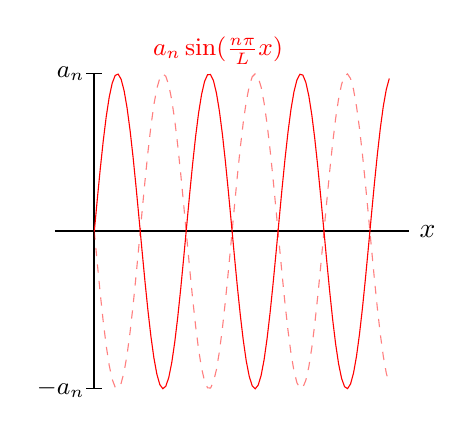
\begin{tikzpicture}
% Axis
\draw[thick] (-.5,0)--(4,0) node[right]{$x$};
\draw[thick] (0,-2)--(0,2) node[above]{ };

\draw[red, samples=100, domain=0:pi-1] plot ({1.75*\x},{2*sin(3 * pi * \x r)});
\draw[red, samples=100, domain=0:pi-1, dashed, opacity=0.5] plot ({1.75*\x},{2*-sin(3 * pi  * \x r)});

\node[above, red] at (pi/2,2) {\small $a_n \sin(\frac{n\pi}{L}x)$};


\draw[-] (-0.1,-2) -- (0.1,-2) node[left, pos=0.5] {\small $-a_n$};
\draw[-] (-0.1,2) -- (0.1,2) node[left, pos=0.5] {\small $a_n$};

\end{tikzpicture}
